\documentclass{beamer}


\usepackage{graphicx}
\usepackage{amsmath}
\usepackage{amssymb}
\usepackage{geometry}
\usepackage{adjustbox} % Include this in the preamble

% Choose a theme or remove if you want the default
\usetheme{Madrid}

\usepackage{algorithm}
\usepackage{algorithmic}

\usepackage[T1]{fontenc}
\usepackage{hyperref}
\usepackage{float}
\usepackage{caption}
\usepackage{subcaption}

% Some optional packages
\usepackage[utf8]{inputenc}
\usepackage[T1]{fontenc}
\usepackage{tikz}
\usetikzlibrary{arrows,shapes,positioning}

% Title, author, date
\title[HoloTax]{\Large HoloTax: A Cryptographic Approach to Reducing Wealth Inequality}
\author{Mamanchuk Mykola, UT, 202420671}
\date{\today}

\begin{document}

%----------------------------------
% Slide 1: Overview
%----------------------------------
\begin{frame}{Context and Overview}
\small
\textbf{Problem Statement:}  
Wealth disparity continues to grow, due in part to corruption, opaque financial channels, and tax avoidance. Traditional taxation methods struggle with enforcement and fairness.

\vspace{0.5em}
\textbf{Proposed Startup: \emph{HoloTax}}  
\begin{itemize}
  \item \textbf{Core Idea:} Use \textcolor{blue}{homomorphic encryption (HE)} and \textcolor{blue}{zero-knowledge proofs (ZKPs)} to ensure fair tax assessment and collection.
  \item \textbf{Smart Contracts:} Automate payments and distribution of tax revenues (e.g., social programs, UBI).
  \item \textbf{Anti-Corruption:} Officials cannot see raw financial data, reducing bribery and favoritism potential.
  \item \textbf{Scalable:} Can integrate with or complement existing government infrastructures.
\end{itemize}

\textbf{Key Benefits:}
\begin{itemize}
  \item Increased \textcolor{blue}{trust} in taxation.
  \item \textcolor{blue}{Greater revenues} for essential social programs.
  \item \textcolor{blue}{Privacy} protection for taxpayers.
\end{itemize}
\end{frame}

%----------------------------------
% Slide 2: Diagram & Process
%----------------------------------
\begin{frame}{System Flow Diagram}
\small

\begin{center}
\scalebox{0.6}{
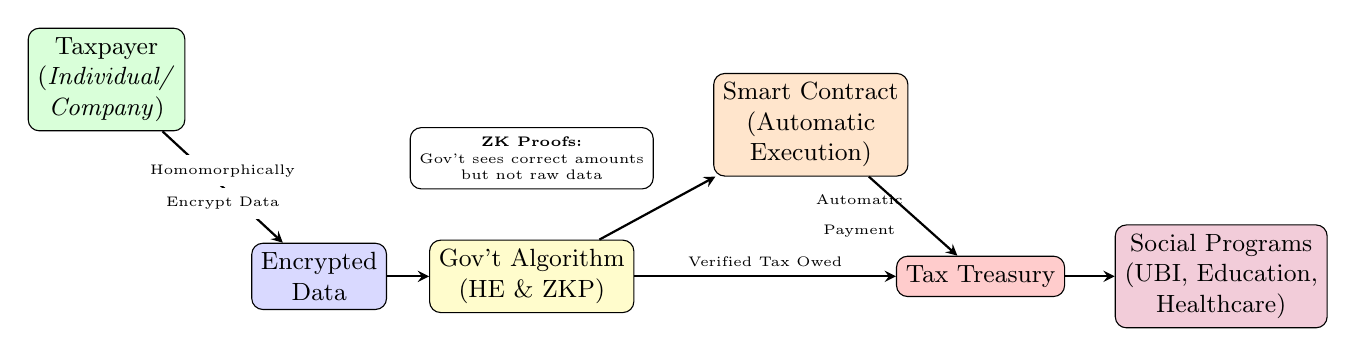
\begin{tikzpicture}[>=stealth, node distance=2.2cm, 
                    every node/.style={align=center, font=\small}]
  % Define nodes
  \node[minimum size=0.5cm , draw, rectangle, rounded corners, fill=green!15] (taxpayer) 
    {Taxpayer\\(\textit{Individual/}\\\textit{Company})};

  \node[draw, rectangle, rounded corners, fill=blue!15, right of=taxpayer, yshift=-25mm, xshift=5mm] (encrypt) 
    {Encrypted\\Data};

  \node[draw, rectangle, rounded corners, fill=yellow!20, right of=encrypt, xshift=5mm] (gov) 
    {Gov’t Algorithm\\(HE \& ZKP)};

  \node[draw, rectangle, rounded corners, fill=orange!20, above right=0.8cm and 1.0cm of gov] (smartc) 
    {Smart Contract\\(Automatic\\ Execution)};

  \node[draw, rectangle, rounded corners, fill=red!20, right of=gov, xshift=35mm] (treasury) 
    {Tax Treasury};

  \node[draw, rectangle, rounded corners, fill=purple!20, right=6.1cm of gov] (social) 
    {Social Programs\\(UBI, Education,\\Healthcare)};

  % Define paths
  \draw[->, thick] (taxpayer) -- node[above, dashed, rectangle, fill=white]{\tiny Homomorphically} 
                            node[below, dashed, rectangle, fill=white]{\tiny Encrypt Data} (encrypt);
  \draw[->, thick] (encrypt) -- (gov);
  \draw[->, thick] (gov) -- node[above]{\tiny Verified Tax Owed}(treasury);
  \draw[->, thick] (gov) -- (smartc);
  \draw[->, thick] (smartc) -- node[left]{\tiny Automatic \\ \tiny Payment}(treasury);
  \draw[->, thick] (treasury) -- (social);

  % Optional callouts
  \node[draw, rectangle, rounded corners, fill=white, font=\tiny, above of=gov, yshift=-0.7cm]
  {\textbf{ZK Proofs:}\\Gov’t sees correct amounts \\ but not raw data};

\end{tikzpicture}
}
\end{center}

\textbf{How It Works:}
\begin{itemize}
  \item \textbf{Encryption:} Taxpayer encrypts financial data; only mathematical operations are allowed on ciphertext.
  \item \textbf{Gov’t Algorithm:} Applies tax code (still in encrypted form), obtains tax liability.
  \item \textbf{Smart Contract:} Ensures automatic payment to treasury and earmarked social funds.
  \item \textbf{Zero-Knowledge:} Government can \emph{verify} data validity \textit{without} learning sensitive details.
\end{itemize}

\end{frame}

\begin{frame}{Little More Details}
    \small
    \textbf{Implementation Path:}
    \begin{itemize}
        \item Launch \textbf{pilot programs} with willing municipalities or large corporations 
              to prove the concept in a controlled environment.
        \item Gradually scale to \textbf{regional/national} adoption once legal frameworks and 
              public trust are established.
    \end{itemize}

    \textbf{Data Governance \& Audit Trails:}
    \begin{itemize}
        \item Encrypted data at rest and in transit, with \textbf{audit logs} for all 
              critical operations (e.g., zero-knowledge proofs, transaction records).
        \item \textbf{Open-source} cryptographic libraries to increase transparency and 
              encourage peer review.
    \end{itemize}

    \textbf{Legal \& Policy Integration:}
    \begin{itemize}
        \item Align with existing \textbf{financial regulations} and eID frameworks where possible.
        \item Engage \textbf{lawmakers and oversight bodies} early to reduce friction in 
              adoption and avoid potential policy conflicts.
    \end{itemize}
\end{frame}


\begin{frame}{Hardships to Tackle}
    \small
    \textbf{Challenges:}
    \begin{itemize}
      \item Computational complexity of HE.
      \item Political and legal hurdles.
      \item User education and acceptance.
    \end{itemize}
\end{frame}

\end{document}
